\chapter{Ergebnisse}
\label{sec:ergebnisse}

Im folgenden Protokollabschnitt werden die Versuchsergebnisse der Versuchsdurchführung präsentiert.
\vspace*{-3.5mm}

\section{Sedimentationsverhalten}
\section{Absetzvolumen}
\section{Trockensubstanz TS}
\section{organische Trockensubstanz oTS}
\section{chemischer Sauerstoffbedarf CSB}
\section{biologischer Sauerstoffbedarf BSB$_5$}

\newpage

\section{Gegenüberstellung der Mindestanforderungen für das Einleiten kommunaler Abwässer in einen Vorfluter der GK 5 mit den Abwasserproben}
Die Referenzwerte der Mindestanforderungen für das Einleiten kommunaler Abwässer in den Vorfluter der Größenklasse 5 sind im Anhang von \cite[S. 29]{Skript} zu finden.
\vspace*{-2.5mm}
\renewcommand{\arraystretch}{1.2}
\begin{table}[h!]
	\centering
	\caption{Tabellarischer Vergleich der Messwerte mit den Mindestanforderungen für das Einleiten kommunaler Abwässer in den Vorfluter der GK 5}
	\label{tab_vgl}
	%\resizebox{10cm}{!}{
	\begin{tabulary}{1.2\textwidth}{l|C|C}
		\hline
		 & \textbf{$CSB$} $\boldsymbol{\left[\si{\milli\gram\per\liter}\right]}$ & \textbf{$BSB_5$} $\boldsymbol{\left[\si{\milli\gram\per\liter}\right]}$\\
		\hline
		\textbf{Grenzwert} & \textbf{75} & \textbf{15}  \\
		\hline
		Probe 1 &  &  \\
		Probe 2 &  &  \\
		Probe 3 &  &  \\
		\hline
	\end{tabulary}
	%}
\end{table}
\FloatBarrier

\begin{figure}[h!]
	\begin{tikzpicture}
	\selectcolormodel{gray}
	\begin{axis}[
	xbar=1pt,% space of 0pt between adjacent bars
	bar width=7,
	width=15cm,
	height=7cm,
	%minor y tick num=4,
	xmax=90,xmin=0,
	x tick label style={/pgf/number format/.cd,%
		scaled x ticks = false,
		set decimal separator={,},
		fixed},
	symbolic y coords={Probe 3,Probe 2,Probe 1,max. für GK 5},
	ytick=data,
	%legend style={at={(0.5,-0.15)},
	%	anchor=north,legend columns=-1},
	xtick={0,10,...,90},
	grid=major,
	xlabel=Gehalt in  \si{\milli\gram\per\liter},
	%enlargelimits=0.15,
	%postaction={pattern=north east lines}
	]
	%CSB
	\addplot[fill=black] coordinates {
		(0,Probe 1) (1.3,Probe 2) (0.6,Probe 3) (75,max. für GK 5)
	};
	%BSB5
	\addplot coordinates {
		(50,Probe 1) (0.77,Probe 2) (2.18,Probe 3) (15,max. für GK 5)
	};

	\legend{$CSB$,$BSB_5$}
	\end{axis}
	\end{tikzpicture}
	\caption{Vergleich mit Mindestanforderungen für das Einleiten kommunaler Abwässer in den Vorfluter der GK 5 für die Abwasserproben 1 bis 3}
	\label{Balkendiagramm}
\end{figure}
\FloatBarrier


\newpage

\section{Gegenüberstellung der durchschnittlichen Beschaffenheit von häuslichem Abwasser mit den Abwasserproben}

Um die Messwerte des Versuches mit häuslichem Abwasser gegenüberzustellen wird die Tabelle Tab. \ref{tab:komm} (siehe \cite[S. 29]{Skript}) genutzt.

\vspace*{0.5cm}
\renewcommand{\arraystretch}{1.2}
\begin{table}[h!]
	\centering
	\caption[Tabellenausschnitt zur durchschnittlichen Beschaffenheit von häuslichem Abwasser]{Tabellenausschnitt zur durchschnittlichen Beschaffenheit von häuslichem Abwasser \cite[S. 29]{Skript}}
	\label{tab:komm}
	%\resizebox{10cm}{!}{
	\begin{tabulary}{1.2\textwidth}{l|C|C|C|C}
	\textbf{Kriterium} 		& \textbf{Maßeinheit} 				&\multicolumn{3}{c}{\textbf{Belastungsgrad}}\\
	\hline
							&									& gering	& mittel & stark\\
	\hline
	Absetzbare Stoffe		&\si{\milli \liter \per \liter} 	& 2			& 6	 	 & 12\\
	Abfiltrierbare Stoffe	&\si{\milli \gram \per \liter} 		& 200		&500	 & 900\\
	$CSB$					&\si{\milli \gram \per \liter} 		& 300		&600	 & 1000\\
	$BSB_5$					&\si{\milli \gram \per \liter}		& 150		&300	 & 500\\
	\end{tabulary}
	%}
\end{table}
\FloatBarrier
\vspace*{1.5cm}

\begin{figure}[h!]
	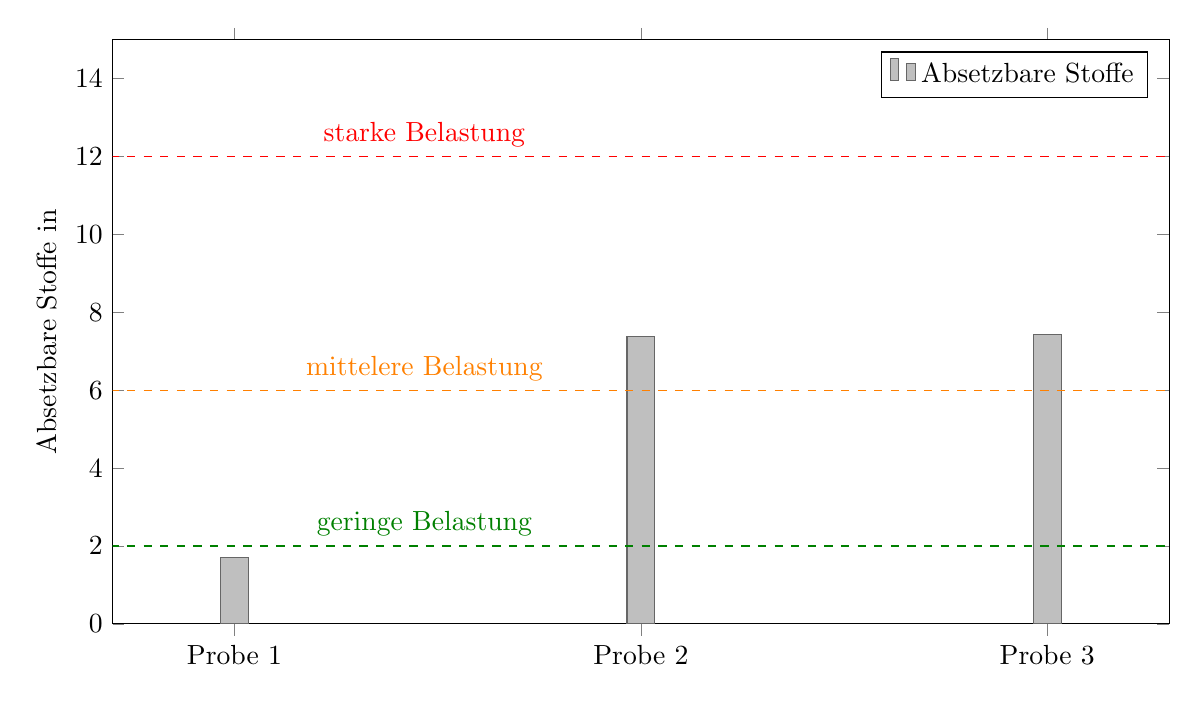
\begin{tikzpicture}
	\begin{axis}[
	%x tick label style={
	%	/pgf/number format/1000 sep=},
	xtick = data,
	ylabel=Absetzbare Stoffe in \si{\milli \liter \per \liter},
   	enlarge x limits=0.15,
	ybar,
	ymin = 0,
	ymax = 15,
	bar width=10pt,
	width=15cm,
	height=9cm,
	symbolic x coords={0,Probe 1, Probe 2,Probe 3,2,1},
	]
	\addplot[fill=gray!50,draw=black!60] coordinates {(Probe 1,1.7) (Probe 2,7.38) (Probe 3,7.44)
	};
	\addplot[green!50!black,sharp plot,update limits=false, dashed] 
	coordinates {(0,2) (1,2)} 
	node[above] at (axis cs:Probe 2,2) {\hspace*{-5.5cm}geringe Belastung
	};
	\addplot[orange,sharp plot,update limits=false, dashed] 
	coordinates {(0,6) (1,6)} 
	node[above] at (axis cs:Probe 2,6) {\hspace*{-5.5cm}mittelere Belastung
	};
	\addplot[red,sharp plot,update limits=false, dashed] 
	coordinates {(0,12) (1,12)} 
	node[above] at (axis cs:Probe 2,12) {\hspace*{-5.5cm}starke Belastung
	};
	\legend{Absetzbare Stoffe}
	\end{axis}
	\end{tikzpicture}
	\caption{Absetzbare Stoffe der Abwasserproben 1 bis 3}
	\label{dia:absetz}
\end{figure}
\FloatBarrier

\begin{figure}[h!]
	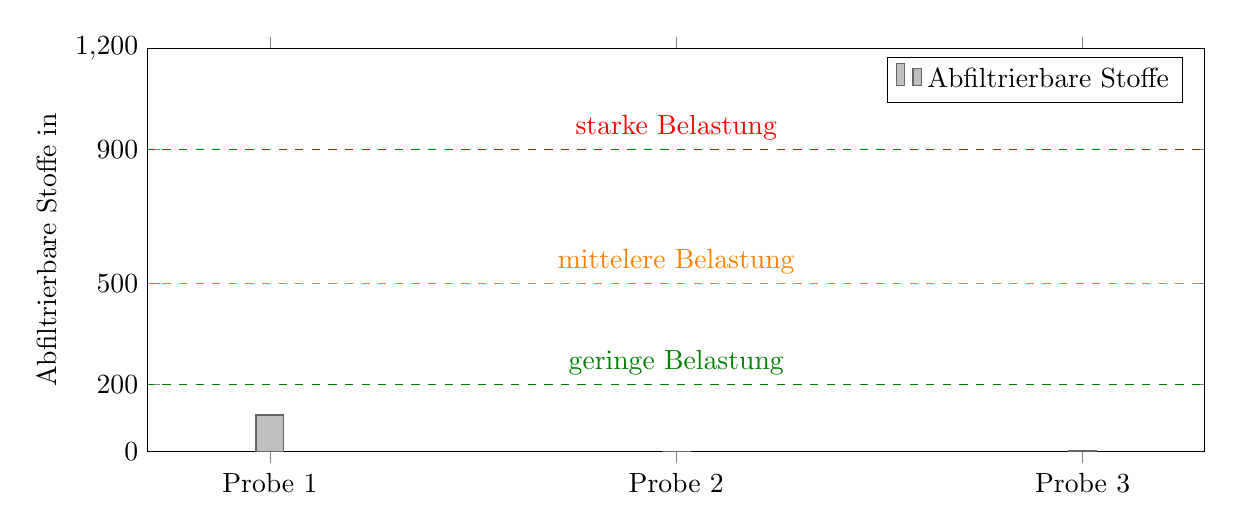
\begin{tikzpicture}
	\begin{axis}[
	%x tick label style={
	%	/pgf/number format/1000 sep=},
	xtick = data,
	ylabel=Abfiltrierbare Stoffe in \si{\milli \gram \per \liter},
	enlarge x limits=0.15,
	ybar,
	ymin = 0,
	ymax = 1200,
	ytick ={0,200,500,900,1200},
	bar width=10pt,
	width=15cm,
	height=6.7cm,
	symbolic x coords={0,Probe 1, Probe 2,Probe 3,2,1},
	]
	\addplot[fill=gray!50,draw=black!60] coordinates {(Probe 1,108.7) (Probe 2,0.77) (Probe 3,2.18)
	};
	\addplot[green!50!black,sharp plot,update limits=false, dashed] 
	coordinates {(0,200) (1,200)} 
	node[above] at (axis cs:Probe 2,200) {geringe Belastung
	};
	\addplot[orange,sharp plot,update limits=false, dashed] 
	coordinates {(0,500) (1,500)} 
	node[above] at (axis cs:Probe 2,500) {mittelere Belastung
	};
	\addplot[red,sharp plot,update limits=false, dashed] 
	coordinates {(0,900) (1,900)} 
	node[above] at (axis cs:Probe 2,900) {starke Belastung
	};
	\legend{Abfiltrierbare Stoffe}
	\end{axis}
	\end{tikzpicture}
	\caption{Abfiltrierbare Stoffe der Abwasserproben 1 bis 3}
	\label{dia:abfilt}
\end{figure}
\FloatBarrier

\begin{figure}[h!]
	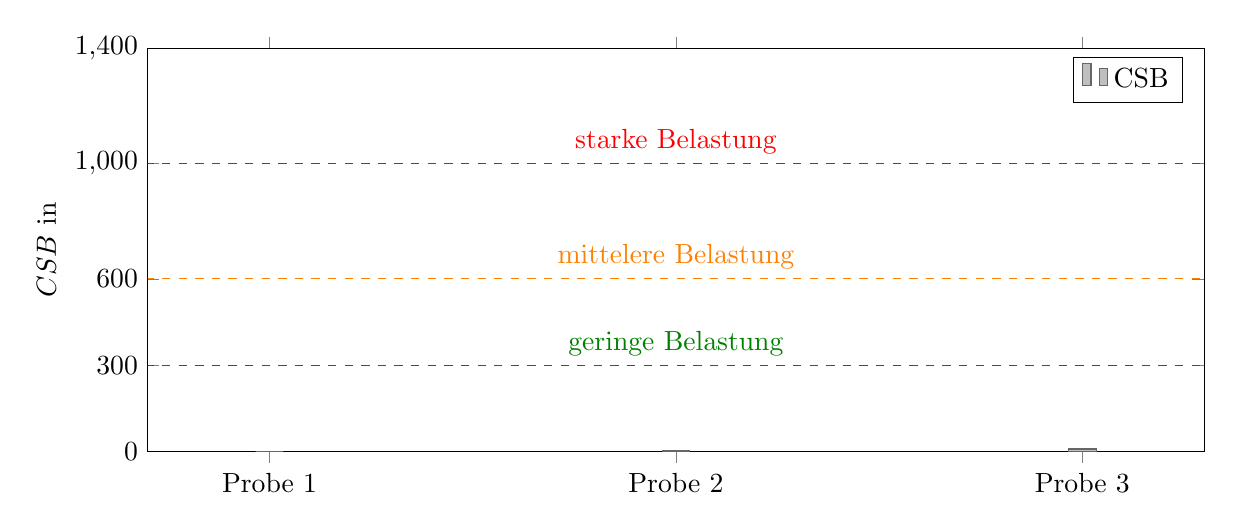
\begin{tikzpicture}
	\begin{axis}[
	%x tick label style={
	%	/pgf/number format/1000 sep=},
	xtick = data,
	ylabel=$CSB$ in \si{\milli \gram \per \liter},
	enlarge x limits=0.15,
	ybar,
	ymin = 0,
	ymax = 1400,
	ytick ={0,300,600,1000,1400},
	bar width=10pt,
	width=15cm,
	height=6.7cm,
	symbolic x coords={0,Probe 1, Probe 2,Probe 3,2,1},
	]
	\addplot[fill=gray!50,draw=black!60] coordinates {(Probe 1,0) (Probe 2,3.9) (Probe 3,8.8)
	};
	\addplot[green!50!black,sharp plot,update limits=false, dashed] 
	coordinates {(0,300) (1,300)} 
	node[above] at (axis cs:Probe 2,300) {geringe Belastung
	};
	\addplot[orange,sharp plot,update limits=false, dashed] 
	coordinates {(0,600) (1,600)} 
	node[above] at (axis cs:Probe 2,600) {mittelere Belastung
	};
	\addplot[red,sharp plot,update limits=false, dashed] 
	coordinates {(0,1000) (1,1000)} 
	node[above] at (axis cs:Probe 2,1000) {starke Belastung
	};
	\legend{CSB}
	\end{axis}
	\end{tikzpicture}
	\caption{Chemischer Sauerstoffbedarf (CSB) der Abwasserproben 1 bis 3}
	\label{dia:csb}
\end{figure}
\FloatBarrier

\begin{figure}[h!]
	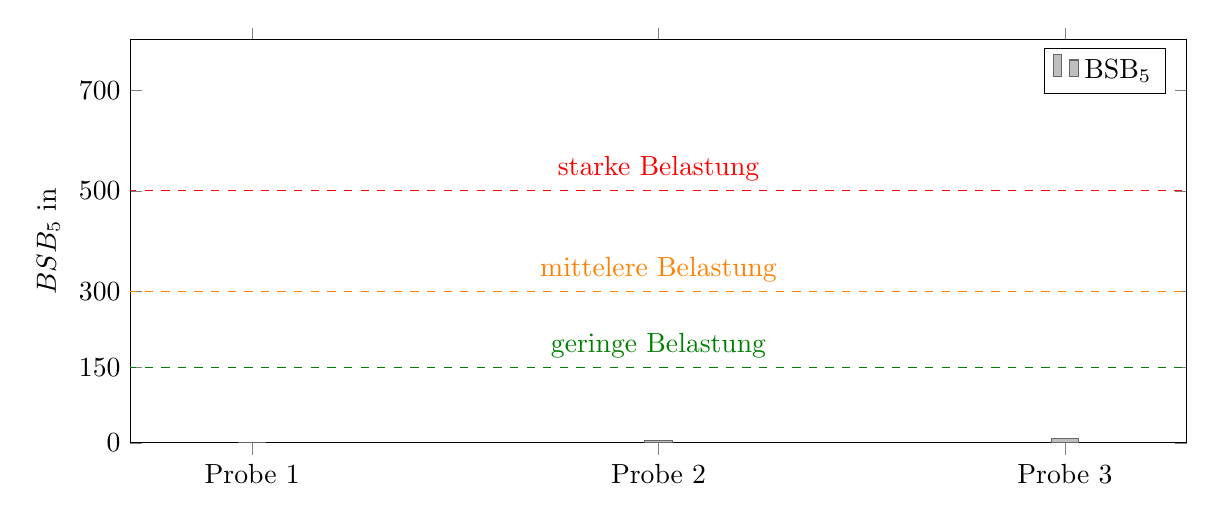
\begin{tikzpicture}
	\begin{axis}[
	%x tick label style={
	%	/pgf/number format/1000 sep=},
	xtick = data,
	ylabel=$BSB_5$ in \si{\milli \gram \per \liter},
	enlarge x limits=0.15,
	ybar,
	ymin = 0,
	ymax = 800,
	ytick ={0,150,300,500,700},
	bar width=10pt,
	width=15cm,
	height=6.7cm,
	symbolic x coords={0,Probe 1, Probe 2,Probe 3,2,1},
	]
	\addplot[fill=gray!50,draw=black!60] coordinates {(Probe 1,0) (Probe 2,3.9) (Probe 3,8.8)
	};
	\addplot[green!50!black,sharp plot,update limits=false, dashed] 
	coordinates {(0,150) (1,150)} 
	node[above] at (axis cs:Probe 2,150) {geringe Belastung
	};
	\addplot[orange,sharp plot,update limits=false, dashed] 
	coordinates {(0,300) (1,300)} 
	node[above] at (axis cs:Probe 2,300) {mittelere Belastung
	};
	\addplot[red,sharp plot,update limits=false, dashed] 
	coordinates {(0,500) (1,500)} 
	node[above] at (axis cs:Probe 2,500) {starke Belastung
	};
	\legend{BSB$_5$}
	\end{axis}
	\end{tikzpicture}
	\caption{Biochemischer Sauerstoffbedarf über 5 Tage (BSB$_5$) der Abwasserproben 1 bis 3}
	\label{dia:bsb}
\end{figure}
\FloatBarrier

